\section{Stavy nabídky}
\label{nur:status}

Nabídka může být v~jednom z~pěti stavů:
\begin{itemize}
    \item \textbf{Čeká na druhého uživatele} -- Nabídka byla vytvořena a čeká na druhého účastníka nabídky.
    \item \textbf{Čeká na schválení} -- Nabídka již má oba účastníky směny a momentálně čeká na schválení uživatele uživatelem, který nabídku vytvořil.
    \item \textbf{Připravena ke směně} -- V~tomto momentě jsou zobrazeny kontaktní údaje a uživatelé se domlouvají na směně peněz.
    \item \textbf{Dokončená} -- Nabídka je kompletní.
    \item \textbf{Smazaná} -- Nabídka byla smazána uživatelem, který ji vytvořil.
\end{itemize}
Jak lze přecházet ze stavu do stavu znázorňuje stavový diagram \ref{fig:implementation:state-diagram}.
\begin{figure}[h]
    \centering
    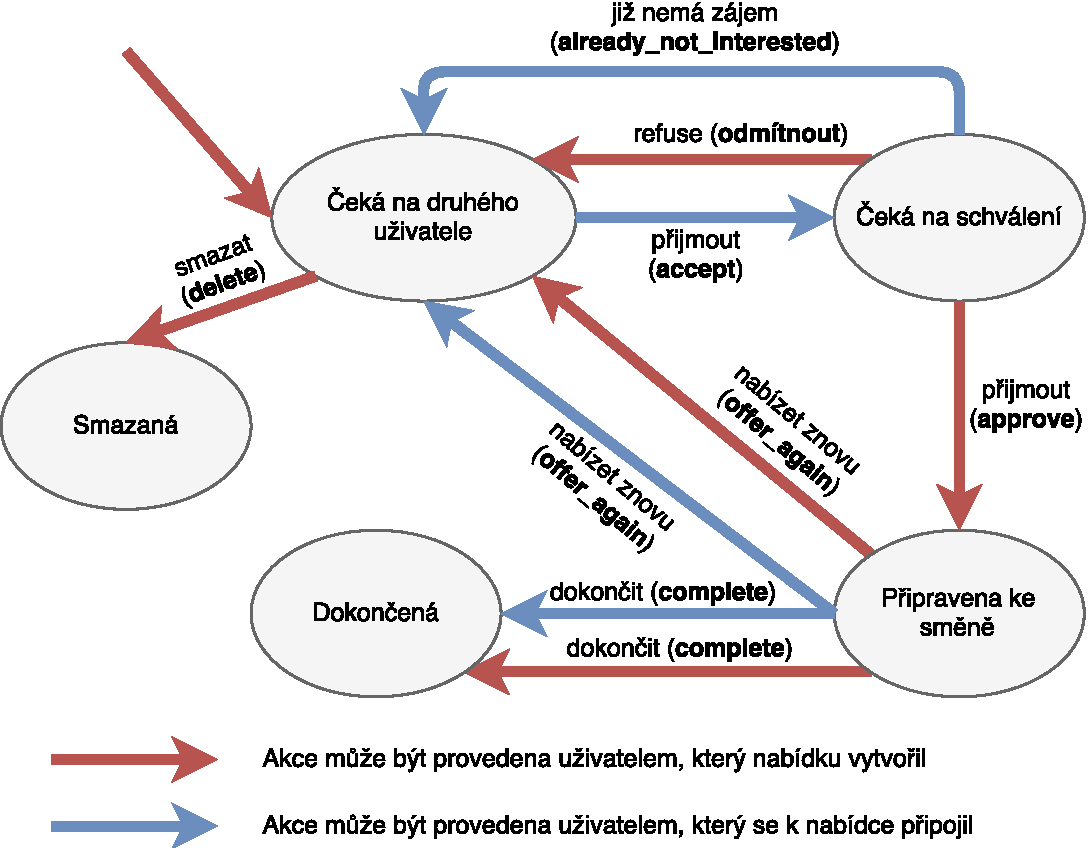
\includegraphics[width=1.0\textwidth]{media/state-diagram-cs}
    \caption{Stavový diagram nabídky}
    \label{fig:implementation:state-diagram}
\end{figure}

Se změnami stavů objednávky úzce souvisí odesílání e-mailů uživatelům.